\documentclass[pdflatex,sn-mathphys-num]{sn-jnl}

\usepackage{graphicx}
\usepackage{amsmath,amssymb}
\usepackage{booktabs}
\usepackage{array}
\usepackage{tabularx}
\usepackage{multirow}
\usepackage{xcolor}
\usepackage{manyfoot}
\usepackage{tikz}
\usetikzlibrary{arrows.meta,positioning,fit,calc,shapes.geometric}

\raggedbottom

\begin{document}

\title[Explainable NER for Low-Resource Languages]{Explainable Named Entity Recognition for Low-Resource Languages Using Attention Attribution}

\author*[1]{\fnm{First} \sur{Author}}\email{author@university.edu}
\affil*[1]{\orgdiv{Department of Computer Science and Engineering}, \orgname{University Research Laboratory}, \orgaddress{\country{India}}}

\abstract{This document presents Section 6 (Methodology) of the research paper entitled ``Explainable Named Entity Recognition for Low-Resource Languages Using Attention Attribution''. The methodology outlines the complete from-scratch data processing, neural architecture, multi-stage training schedule, and explainability framework across four low-resource languages: Konkani, Assamese, Sinhala, and Kokborok.}

\keywords{Named Entity Recognition, Low-Resource Languages, Attention Attribution, Character CNN, BiLSTM-CRF, Faithfulness Evaluation}

\maketitle

\section{Methodology}\label{sec:methodology}

This section describes the methodology used to develop and evaluate an explainable named entity recognition (NER) system for four low-resource languages: Konkani, Assamese, Sinhala, and Kokborok. The system is designed under a strict constraint: all models, embeddings, and tokenizers are constructed and trained entirely from scratch. No external pretrained language models (such as BERT, mBERT, XLM-RoBERTa, MuRIL, or IndicBERT) and no external static word embeddings (such as FastText or Word2Vec) are used anywhere in the pipeline.

The following subsections describe the dataset preparation, the preprocessing pipeline, the overall research framework, the proposed neural architecture, the baseline configurations, the mathematical formulation, the multi-stage training procedure, and the explainability and faithfulness evaluation methods.

\subsection{Data Collection and Dataset Preparation}\label{subsec:data_prep}

The target languages represent four distinct linguistic and orthographic environments:
\begin{enumerate}
    \item \textbf{Konkani} (\textit{gom}): An Indo-Aryan language spoken along the western coast of India, written here in the Devanagari script.
    \item \textbf{Assamese} (\textit{as}): An Eastern Indo-Aryan language spoken in Assam, India, written in the Assamese-Bengali script.
    \item \textbf{Sinhala} (\textit{si}): An Indo-Aryan language of Sri Lanka, written in the Sinhala script with distinctive syllabic conjuncts.
    \item \textbf{Kokborok}: A Tibeto-Burman language of Tripura, India, written here in the Roman script.
\end{enumerate}

Raw text for Konkani, Assamese, and Sinhala was gathered from public Wikipedia archives and regional digital newspapers. Konkani sources include the Konkani Wikipedia, Herald Goa, and Bhaangarbhuin. Assamese sources include the Assamese Wikipedia, Asomiya Pratidin, and Niyomiya Barta. Sinhala sources include the Sinhala Wikipedia, Ada Derana Sinhala, and Dinamina. The collected documents were filtered to remove noise and low-script purity segments, and deduplicated using SHA-256 document hashing. For Kokborok, raw data was compiled from public corpora into a unified collection of 20,300 sentence pairs.

Annotated corpora were developed using structured heuristic and dictionary-based annotation pipelines. Entity boundaries and types were generated algorithmically using gazetteers, orthographic dictionaries, and regular expression patterns. The resulting annotated sentences were formatted into standard CoNLL format.

The annotation schema covers four standard named entity types:
\begin{itemize}
    \item \textbf{PER}: Person names.
    \item \textbf{LOC}: Locations and geopolitical entities.
    \item \textbf{ORG}: Organizations, companies, and institutions.
    \item \textbf{MISC}: Miscellaneous named entities outside the first three categories.
\end{itemize}

Labels are encoded using the standard BIO (Beginning, Inside, Outside) tagging scheme. This produces nine possible token-level classes: O, B-PER, I-PER, B-LOC, I-LOC, B-ORG, I-ORG, B-MISC, and I-MISC.

Each language dataset was partitioned into three disjoint splits: training, development, and Gold-Test. The Gold-Test sets were strictly protected throughout model development: they were not used for training, were not used for hyperparameter tuning, and remained locked while models were being developed. Gold-Test evaluations were executed only after model checkpoints were finalized and frozen. To guarantee dataset integrity, the test sets were protected using SHA-256 checksums, which were recorded prior to evaluation and verified to ensure that test data had remained unmodified. Table~\ref{tab:dataset} reports the verified dataset characteristics and split sizes.

\begin{table}[htbp]
\centering
\caption{Dataset Characteristics and Gold-Test Distribution across the Four Target Languages}
\label{tab:dataset}
\small
\begin{tabular}{lllllll}
\toprule
\textbf{Language} & \textbf{Script} & \textbf{Raw Data Sources} & \textbf{Training} & \textbf{Dev.} & \textbf{Gold Test} & \textbf{Other Data} \\
\midrule
Konkani  & Devanagari       & Wikipedia, Herald Goa, Bhaangarbhuin & 850 sents. & 200 sents. & 200 sents. (124 ent.) & --- \\
Assamese & Assamese-Bengali & Wikipedia, Asomiya Pratidin, Niyomiya Barta & 850 sents. & 200 sents. & 200 sents. (138 ent.) & --- \\
Sinhala  & Sinhala          & Wikipedia, Ada Derana, Dinamina & 850 sents. & 200 sents. & 200 sents. (132 ent.) & --- \\
Kokborok & Roman            & Public corpus (20,300 sentence pairs) & 849 sents. & 199 sents. & 199 sents. (16 ent.)  & Exp. 10--11 public corpus \\
\bottomrule
\end{tabular}
\end{table}

As shown in Table~\ref{tab:dataset}, the Kokborok Gold-Test set contains 16 annotated entities across 199 sentences, whereas the test sets for Konkani, Assamese, and Sinhala contain between 124 and 138 entities across 200 sentences. Because the Kokborok test set has a lower entity density, every individual entity prediction produces a larger percentage change in the precision, recall, and F1 metrics for that language.

\subsection{Preprocessing and Grapheme-Level Tokenization}\label{subsec:preprocessing}

Raw text from all four languages was processed through a unified text normalization and tokenization pipeline implemented entirely from scratch.

\textbf{Unicode NFC Normalization.} All text was normalized to Unicode Normalization Form C (NFC). In South Asian scripts, the same visible character sequence can frequently be encoded in multiple distinct ways (for example, as a precomposed character or as a base character followed by combining vowel marks). Canonical NFC normalization maps equivalent representations to a single unique byte sequence. Invisible formatting characters, byte-order marks, and zero-width spaces (\texttt{U+200B}) were removed. Zero-Width Joiner (ZWJ, \texttt{U+200D}) and Zero-Width Non-Joiner (ZWNJ, \texttt{U+200C}) characters were retained because they are required to form correct conjunct consonants in Devanagari, Assamese-Bengali, and Sinhala.

\textbf{Sinhala Conjunct Repair.} Sinhala digital text frequently contains damaged conjunct ligatures caused by inconsistent font encoding. A rule-based repair pass was applied prior to normalization to restore missing ZWJ characters between consonant virama combinations and touching letters (\textit{bandi akshara}).

\textbf{Word Tokenization.} Text was split into word tokens using a rule-based tokenizer based on Unicode character classes. The tokenizer groups contiguous sequences of letters, combining marks, numbers, and joiners into single word tokens while isolating punctuation marks. This prevents accidental splitting of dependent vowel signs from their consonant bases.

\textbf{Grapheme-Level Segmentation.} To obtain fine-grained character representations without breaking orthographic units, words were segmented into extended grapheme clusters using the \texttt{\textbackslash X} pattern. In Brahmic writing systems, an extended grapheme cluster corresponds to an orthographic syllable (\textit{akshara}), consisting of a base consonant, optional virama-consonant conjuncts, dependent vowel signs, and modifiers:
\[
\text{Grapheme Cluster} = \text{Consonant} \cdot (\text{Virama} \cdot \text{Consonant})^* \cdot \text{Vowel\_Sign}^* \cdot \text{Modifier}^*.
\]
In simple terms, this formula defines a complete visual syllable by attaching vowel signs and modifiers to a base consonant cluster. Here, the dot denotes string concatenation, and the asterisk indicates zero or more occurrences. Treating each cluster as a single unit prevents the subword fragmentation that occurs when standard subword tokenizers divide characters across byte boundaries.

\subsection{Overall Research Framework}\label{subsec:framework}

The research framework follows a sequential pipeline comprising nine distinct stages. Figure~\ref{fig:framework} illustrates the overall workflow.

\begin{figure*}[t]
\centering
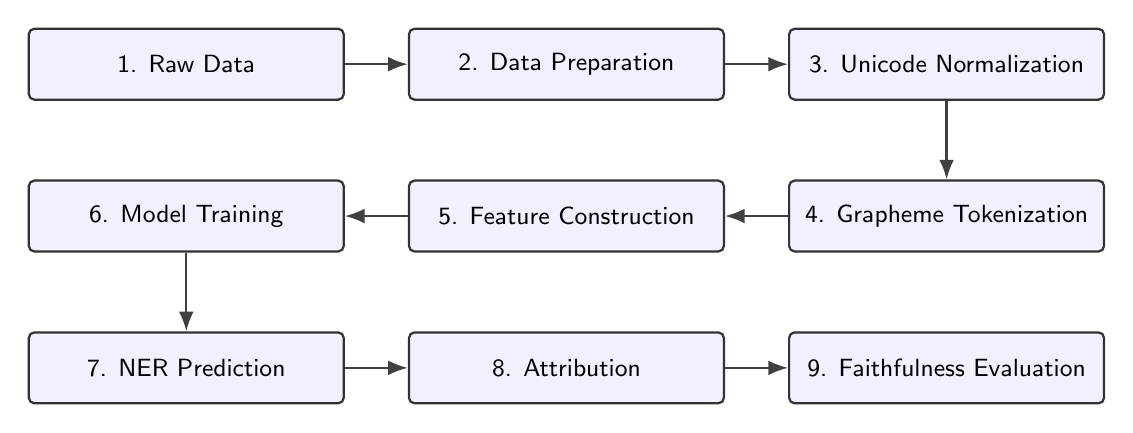
\begin{tikzpicture}[
    node distance=10mm and 8mm,
    stage/.style={
        rectangle,
        rounded corners=2pt,
        draw=black!80,
        fill=blue!6,
        thick,
        align=center,
        font=\small\sffamily,
        minimum width=4.0cm,
        minimum height=0.9cm
    },
    arrow/.style={
        -{Latex[length=2.5mm]},
        thick,
        draw=black!75
    }
]

% Row 1: Stages 1 to 3
\node[stage] (s1) {1. Raw Data};
\node[stage, right=of s1] (s2) {2. Data Preparation};
\node[stage, right=of s2] (s3) {3. Unicode Normalization};

% Row 2: Stages 4 to 6
\node[stage, below=of s3] (s4) {4. Grapheme Tokenization};
\node[stage, left=of s4] (s5) {5. Feature Construction};
\node[stage, left=of s5] (s6) {6. Model Training};

% Row 3: Stages 7 to 9
\node[stage, below=of s6] (s7) {7. NER Prediction};
\node[stage, right=of s7] (s8) {8. Attribution};
\node[stage, right=of s8] (s9) {9. Faithfulness Evaluation};

% Connectors Row 1
\draw[arrow] (s1) -- (s2);
\draw[arrow] (s2) -- (s3);

% Transition Row 1 -> Row 2
\draw[arrow] (s3.south) -- (s4.north);

% Connectors Row 2
\draw[arrow] (s4) -- (s5);
\draw[arrow] (s5) -- (s6);

% Transition Row 2 -> Row 3
\draw[arrow] (s6.south) -- (s7.north);

% Connectors Row 3
\draw[arrow] (s7) -- (s8);
\draw[arrow] (s8) -- (s9);

\end{tikzpicture}
\caption{Overall research framework showing the nine sequential stages of the experimental pipeline. Stages 8 (Attribution) and 9 (Faithfulness Evaluation) are conducted separately to assess model interpretability without modifying model parameters.}
\label{fig:framework}
\end{figure*}

The workflow operates as follows:
\begin{enumerate}
    \item \textbf{Raw Data}: Harvesting unstructured text from news and web sources across the four languages.
    \item \textbf{Data Preparation}: Applying heuristic annotation and partitioning into train, dev, and locked test splits.
    \item \textbf{Unicode Normalization}: Enforcing NFC canonical form and repairing script-specific conjuncts.
    \item \textbf{Grapheme Tokenization}: Segmenting words into extended grapheme clusters using the \texttt{\textbackslash X} pattern.
    \item \textbf{Feature Construction}: Building randomly initialized word embeddings, character CNN representations, and language embeddings.
    \item \textbf{Model Training}: Executing multilingual joint training followed by phased layer-wise unfreezing fine-tuning.
    \item \textbf{NER Prediction}: Decoding globally consistent BIO label sequences using the shared linear-chain CRF.
    \item \textbf{Attribution}: Computing Gradient $\times$ Attention scores for predicted entity tokens post-hoc on the frozen model.
    \item \textbf{Faithfulness Evaluation}: Measuring the change in model prediction confidence under top-$k$ versus random-$k$ token erasure.
\end{enumerate}

Stages 8 and 9 are separated deliberately: Stage 8 calculates attribution scores, while Stage 9 experimentally tests whether those scores reflect tokens that influence the model's confidence.

\subsection{Proposed Model Architecture}\label{subsec:architecture}

The proposed model (Model 4) is a language-conditioned, neural sequence labeling architecture trained from scratch. The model combines word-level lexical information, subword character-level morphological features, and source language conditioning into a unified representation. Figure~\ref{fig:architecture} presents the architecture. Table~\ref{tab:architecture} provides layer specifications.

\begin{figure*}[t]
\centering
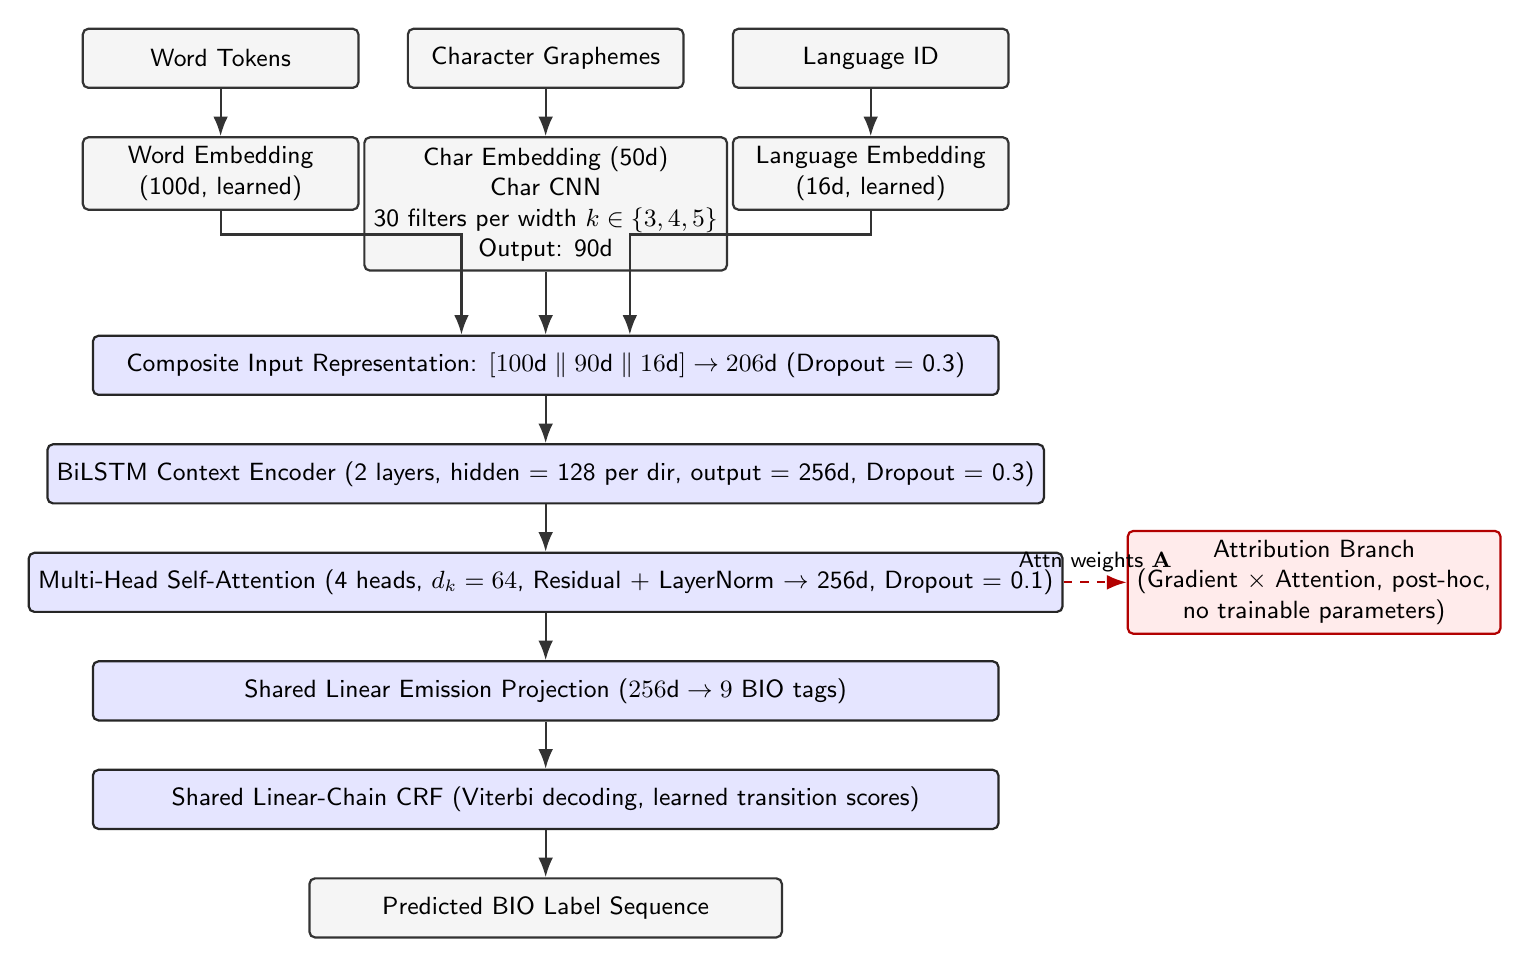
\begin{tikzpicture}[
    node distance=6mm and 6mm,
    block/.style={
        rectangle,
        rounded corners=2pt,
        draw=black!80,
        fill=gray!8,
        thick,
        align=center,
        font=\small\sffamily,
        minimum width=3.5cm,
        minimum height=0.75cm
    },
    accentblock/.style={
        rectangle,
        rounded corners=2pt,
        draw=black!85,
        fill=blue!10,
        thick,
        align=center,
        font=\small\sffamily,
        minimum width=11.5cm,
        minimum height=0.75cm
    },
    explainblock/.style={
        rectangle,
        rounded corners=2pt,
        draw=red!70!black,
        fill=red!8,
        thick,
        align=center,
        font=\small\sffamily,
        minimum width=4.5cm,
        minimum height=0.85cm
    },
    arrow/.style={
        -{Latex[length=2.5mm]},
        thick,
        draw=black!80
    },
    dashedarrow/.style={
        -{Latex[length=2.5mm]},
        thick,
        draw=red!70!black,
        dashed
    }
]

% Top Inputs
\node[block] (in_word) {Word Tokens};
\node[block, right=of in_word] (in_char) {Character Graphemes};
\node[block, right=of in_char] (in_lang) {Language ID};

% Input Embeddings
\node[block, below=of in_word] (emb_word) {Word Embedding\\(100d, learned)};
\node[block, below=of in_char] (emb_char) {Char Embedding (50d) \\
Char CNN \\
30 filters per width $k \in \{3,4,5\}$ \\
Output: 90d};
\node[block, below=of in_lang] (emb_lang) {Language Embedding\\(16d, learned)};

% Combined Representation
\node[accentblock, below=8mm of emb_char] (concat) {Composite Input Representation: $[100\text{d} \parallel 90\text{d} \parallel 16\text{d}] \to 206\text{d}$ (Dropout = 0.3)};

% Sequence Encoder
\node[accentblock, below=of concat] (bilstm) {BiLSTM Context Encoder (2 layers, hidden = 128 per dir, output = 256d, Dropout = 0.3)};

% Multi-Head Self-Attention
\node[accentblock, below=of bilstm] (attn) {Multi-Head Self-Attention (4 heads, $d_k=64$, Residual + LayerNorm $\to$ 256d, Dropout = 0.1)};

% Explainability Branch (Side)
\node[explainblock, right=8mm of attn] (attrib) {Attribution Branch\\(Gradient $\times$ Attention, post-hoc,\\no trainable parameters)};

% Decoder
\node[accentblock, below=of attn] (emission) {Shared Linear Emission Projection ($256\text{d} \to 9\text{ BIO tags}$)};
\node[accentblock, below=of emission] (crf) {Shared Linear-Chain CRF (Viterbi decoding, learned transition scores)};
\node[block, below=of crf, minimum width=6cm] (output) {Predicted BIO Label Sequence};

% Arrows
\draw[arrow] (in_word) -- (emb_word);
\draw[arrow] (in_char) -- (emb_char);
\draw[arrow] (in_lang) -- (emb_lang);

\draw[arrow] (emb_word.south) -- ++(0,-3mm) -| (concat.160);
\draw[arrow] (emb_char.south) -- (concat.north);
\draw[arrow] (emb_lang.south) -- ++(0,-3mm) -| (concat.20);

\draw[arrow] (concat) -- (bilstm);
\draw[arrow] (bilstm) -- (attn);
\draw[arrow] (attn) -- (emission);
\draw[dashedarrow] (attn.east) -- node[above, font=\footnotesize\sffamily] {Attn weights $\mathbf{A}$} (attrib.west);
\draw[arrow] (emission) -- (crf);
\draw[arrow] (crf) -- (output);

\end{tikzpicture}
\caption{Detailed architecture of the proposed multilingual NER model (Model 4). The composite 206-dimensional input vector passes through a 2-layer BiLSTM and a 4-head self-attention layer with residual normalization. The linear emission layer and CRF decoder are shared across all four languages. The attribution branch operates post-hoc on the frozen network.}
\label{fig:architecture}
\end{figure*}

\begin{table}[htbp]
\centering
\caption{Layer-Wise Architecture and Parameter Specifications of the Proposed Model}
\label{tab:architecture}
\small
\begin{tabular}{lllll}
\toprule
\textbf{Layer / Component} & \textbf{Input Dim.} & \textbf{Output Dim.} & \textbf{Configuration} & \textbf{Hyperparameters} \\
\midrule
Word Embedding         & ---    & 100d  & Randomly initialized table & Dropout = 0.3 \\
Char Grapheme Embedding & ---   & 50d   & Extended grapheme clusters & Dropout = 0.3 \\
Char CNN Convolutions  & 50d    & 90d   & Widths $k \in \{3,4,5\}$, 30 filters each & ReLU, global max-pool \\
Language Embedding     & ---    & 16d   & 4 languages, learned table & Learned from scratch \\
Composite Input Vector & ---    & 206d  & Concat: $100\text{d} + 90\text{d} + 16\text{d}$ & Concat Dropout = 0.3 \\
BiLSTM Context Encoder & 206d   & 256d  & 2 layers, hidden = 128 per dir. & Dropout = 0.3 \\
Multi-Head Self-Attn   & 256d   & 256d  & 4 heads, $d_k = 64$, 1 block & Residual + LayerNorm, Drop = 0.1 \\
Linear Emission Proj.  & 256d   & 9d    & Shared linear transformation & Xavier uniform init. \\
Linear-Chain CRF       & 9d     & 9d    & Shared transition matrix & Viterbi decoding \\
\bottomrule
\end{tabular}
\end{table}

\subsubsection{Composite Input Representation}\label{subsubsec:composite_rep}

At each token position $t$, the network forms a composite vector $\mathbf{x}_t$ by concatenating three representations:
\begin{enumerate}
    \item A 100-dimensional word embedding $\mathbf{e}^{(w)}_t$ learned from scratch.
    \item A 90-dimensional character-level representation $\mathbf{e}^{(c)}_t$ generated by the character CNN.
    \item A 16-dimensional language embedding $\mathbf{e}^{(\ell)}$ representing the source language ID.
\end{enumerate}
The resulting vector has 206 dimensions ($100 + 90 + 16 = 206$). A dropout layer with a rate of 0.3 is applied to this vector. This composite representation provides lexical identity through the word vector, morphological cues through the character vector, and language identity through the language embedding.

\subsubsection{Character-Level CNN}\label{subsubsec:char_cnn}

The character CNN extracts morphological information from the grapheme cluster sequence of each word. Each grapheme cluster is mapped to a 50-dimensional learned embedding. Three parallel 1D convolutional layers with kernel widths of 3, 4, and 5 grapheme units are applied. Each kernel width uses 30 filters, followed by a ReLU activation function and global max-over-time pooling. Concatenating the outputs of the three filter sizes yields a 90-dimensional character representation ($3 \times 30 = 90$). This representation allows the model to handle inflected and unseen words that share roots or affixes with known words.

\subsubsection{BiLSTM Context Encoder}\label{subsubsec:bilstm}

The sequence of 206-dimensional vectors is fed into a two-layer bidirectional LSTM. The hidden size is 128 dimensions in each direction. Concatenating the forward hidden state (128d) and backward hidden state (128d) at each token position yields a 256-dimensional contextual vector. A dropout rate of 0.3 is applied to the recurrent outputs. The BiLSTM captures sequential dependencies across the entire sentence.

\subsubsection{Multi-Head Self-Attention}\label{subsubsec:attention}

The BiLSTM representations are processed by a single multi-head self-attention layer with 4 heads. The 256-dimensional space is divided equally across the 4 heads, giving each head a projection dimension of $d_k = 64$. Scaled dot-product attention computes direct interactions between all pairs of tokens in the sentence. The outputs of the 4 heads are concatenated, projected back to 256 dimensions, regularized with an attention dropout of 0.1, and combined with the input through a residual addition followed by Layer Normalization:
\[
\tilde{\mathbf{H}} = \text{LayerNorm}(\mathbf{H} + \text{Dropout}(\text{MultiHead}(\mathbf{H}))).
\]
In simple terms, this equation adds the attention output to the BiLSTM hidden states and normalizes the sum, ensuring stable gradients. Here, $\mathbf{H}$ is the input matrix of hidden states, $\text{MultiHead}(\mathbf{H})$ is the concatenated multi-head context, and $\text{LayerNorm}$ normalizes values across features. This layer allows the model to connect related words across long distances without relying solely on the step-by-step recurrence of the LSTM.

\subsubsection{CRF Decoder}\label{subsubsec:crf}

The attended representations are projected to 9 tag emission scores using a shared linear layer. A shared linear-chain Conditional Random Field (CRF) decodes the label sequence. The shared CRF uses a single transition matrix across all four languages, as confirmed in the final configuration files (\texttt{crf\_config: shared}). During training, the CRF minimizes the negative log-likelihood of the gold label sequence. During inference, the Viterbi decoder selects the highest-scoring complete label sequence using both emission and learned transition scores.

\subsubsection{Explainability Branch}\label{subsubsec:explain_branch}

During the forward pass, the multi-head self-attention module records the attention weight tensors for all four heads. The explainability branch uses these stored weights alongside the model gradients to compute token-level attribution scores after training. This branch adds no trainable parameters and does not change the network's forward predictions.

\subsection{Evaluated Model Configurations}\label{subsec:model_configs}

To study the architectural progression, four model variants were implemented in the project codebase. Table~\ref{tab:models} summarizes their architectural configurations.

\begin{table}[htbp]
\centering
\caption{Evaluated Model Configurations and Architectural Progression}
\label{tab:models}
\small
\begin{tabular}{llll}
\toprule
\textbf{Configuration} & \textbf{Source File} & \textbf{Core Components} & \textbf{Architectural Role} \\
\midrule
Model 1 (Baseline) & \texttt{ner\_model\_v1\_baseline.py} & Word Embed (100d) + BiLSTM + CRF & Word-only baseline \\
Model 2 (Char-CNN) & \texttt{ner\_model\_v2\_charcnn.py}  & Word (100d) + Char-CNN (90d) $\to$ 190d + 2-layer BiLSTM + CRF & Adds character morphology \\
Model 3 (Attention)& \texttt{ner\_model\_v3\_attention.py}& 190d Input + 2-layer BiLSTM + 4-Head Attn + CRF & Adds self-attention mechanism \\
Model 4 (Proposed) & \texttt{ner\_model\_v4\_multilingual.py}& Word (100d) + Char (90d) + Lang (16d) $\to$ 206d + Attn + Shared CRF & Complete multilingual model \\
\bottomrule
\end{tabular}
\end{table}

\textit{Note on Evaluation Evidence:} The project artifacts contain complete, verified Gold-Test evaluation records for the final multilingual system (Model 4). While Models 1, 2, and 3 are implemented in the codebase, separate standalone evaluation logs for these earlier variants are not present in the workspace. Therefore, their individual test F1 scores are not reported here to avoid unverified claims.

\subsubsection{Model 1 --- Word-Level BiLSTM-CRF Baseline}
Model 1 contains a 100-dimensional learned word embedding, a bidirectional LSTM context encoder with hidden size 128 per direction (configured with a single layer by default), a linear emission layer, and a linear-chain CRF decoder. It excludes character embeddings, character convolutions, language conditioning, and self-attention.

\subsubsection{Model 2 --- Char-CNN + BiLSTM-CRF}
Model 2 adds the character CNN to Model 1. The input combines the 100-dimensional word embedding with the 90-dimensional character representation into a 190-dimensional vector. The sequence encoder is expanded to a two-layer BiLSTM followed by a CRF decoder.

\subsubsection{Model 3 --- Char-CNN + BiLSTM + Self-Attention + CRF}
Model 3 adds the 4-head self-attention layer with residual connection and Layer Normalization between the two-layer BiLSTM and the CRF decoder. The input dimension remains 190. This model introduces internal attention weights that can be inspected for explainability.

\subsubsection{Model 4 --- Final Proposed Multilingual Model}
Model 4 adds the 16-dimensional language embedding to Model 3, producing the complete 206-dimensional composite input. The CRF decoder and linear emission projection are shared across all four languages. Model 4 serves as the primary evaluation model.

\subsection{Mathematical Formulation}\label{subsec:math_formulation}

This subsection presents the mathematical definitions for each component of the proposed system.

\subsubsection{Input and Composite Representation}
Let a sentence of $T$ tokens be represented as a sequence of word indices $(w_1, w_2, \ldots, w_T)$, their corresponding grapheme cluster sequences $(\mathbf{c}_1, \mathbf{c}_2, \ldots, \mathbf{c}_T)$, and a language identifier $\ell \in \{0, 1, 2, 3\}$. The composite input vector $\mathbf{x}_t$ at position $t$ is formed by concatenating the word embedding, the character CNN output, and the language embedding:
\begin{equation}
\mathbf{x}_t = [\mathbf{e}^{(w)}(w_t) \parallel \text{CharCNN}(\mathbf{c}_t) \parallel \mathbf{e}^{(\ell)}(\ell)] \in \mathbb{R}^{206}.
\end{equation}
In simple terms, the model joins word information, character information, and language information into one 206-dimensional vector. Here, $\mathbf{e}^{(w)}(w_t) \in \mathbb{R}^{100}$ is the learned word embedding for word $w_t$, $\text{CharCNN}(\mathbf{c}_t) \in \mathbb{R}^{90}$ is the character representation, and $\mathbf{e}^{(\ell)}(\ell) \in \mathbb{R}^{16}$ is the language embedding. The symbol $\parallel$ denotes vector concatenation.

\subsubsection{Character-Level Representation}
For a word with grapheme clusters $(g_1, g_2, \ldots, g_{L})$, each cluster $g_i$ is mapped to a 50-dimensional embedding $\mathbf{e}^{(g)}_i \in \mathbb{R}^{50}$. A 1D convolution with kernel width $k \in \{3, 4, 5\}$ and weight tensor $\mathbf{W}^{(k)} \in \mathbb{R}^{30 \times (k \times 50)}$ computes local features:
\begin{equation}
\mathbf{f}^{(k)}_i = \text{ReLU}\left(\mathbf{W}^{(k)} \cdot \mathbf{e}^{(g)}_{i:i+k-1} + \mathbf{b}^{(k)}\right) \in \mathbb{R}^{30}.
\end{equation}
In simple terms, this operation slides a window of width $k$ across the grapheme embeddings to detect local character patterns. Here, $\mathbf{e}^{(g)}_{i:i+k-1}$ is the concatenated window of $k$ grapheme embeddings, $\mathbf{b}^{(k)} \in \mathbb{R}^{30}$ is a bias term, and $\text{ReLU}(z) = \max(0, z)$ is the activation function. Global max-over-time pooling selects the most salient feature across all window positions:
\begin{equation}
p^{(k)} = \max_{1 \le i \le L - k + 1} \mathbf{f}^{(k)}_i \in \mathbb{R}^{30}.
\end{equation}
In simple terms, pooling keeps only the highest activation for each filter across the entire word. The outputs from all three kernel widths are concatenated:
\begin{equation}
\text{CharCNN}(\mathbf{c}_t) = [p^{(3)} \parallel p^{(4)} \parallel p^{(5)}] \in \mathbb{R}^{90}.
\end{equation}
In simple terms, joining the pooled vectors from widths 3, 4, and 5 forms a complete 90-dimensional morphological summary of the word.

\subsubsection{BiLSTM Context Encoding}
The sequence of input vectors $(\mathbf{x}_1, \ldots, \mathbf{x}_T)$ is processed by a forward LSTM and a backward LSTM:
\begin{equation}
\overrightarrow{\mathbf{h}}_t = \text{LSTM}_{\text{fwd}}(\mathbf{x}_t, \overrightarrow{\mathbf{h}}_{t-1}), \quad
\overleftarrow{\mathbf{h}}_t = \text{LSTM}_{\text{bwd}}(\mathbf{x}_t, \overleftarrow{\mathbf{h}}_{t+1}).
\end{equation}
In simple terms, the forward LSTM reads the sentence from left to right, while the backward LSTM reads it from right to left. The forward hidden state $\overrightarrow{\mathbf{h}}_t \in \mathbb{R}^{128}$ and backward hidden state $\overleftarrow{\mathbf{h}}_t \in \mathbb{R}^{128}$ are concatenated:
\begin{equation}
\mathbf{h}_t = [\overrightarrow{\mathbf{h}}_t \parallel \overleftarrow{\mathbf{h}}_t] \in \mathbb{R}^{256}.
\end{equation}
In simple terms, combining both directions gives each word a 256-dimensional summary of its left and right context. The matrix $\mathbf{H} = (\mathbf{h}_1, \ldots, \mathbf{h}_T)^\top \in \mathbb{R}^{T \times 256}$ collects all hidden states.

\subsubsection{Multi-Head Self-Attention}
For each attention head $h \in \{1, 2, 3, 4\}$, query, key, and value matrices are computed using head-specific projections:
\begin{equation}
\mathbf{Q}^{(h)} = \mathbf{H} \mathbf{W}_Q^{(h)}, \quad
\mathbf{K}^{(h)} = \mathbf{H} \mathbf{W}_K^{(h)}, \quad
\mathbf{V}^{(h)} = \mathbf{H} \mathbf{W}_V^{(h)} \in \mathbb{R}^{T \times 64},
\end{equation}
where $\mathbf{W}_Q^{(h)}, \mathbf{W}_K^{(h)}, \mathbf{W}_V^{(h)} \in \mathbb{R}^{256 \times 64}$. In simple terms, these linear projections transform the BiLSTM representations into queries, keys, and values for head $h$. The scaled dot-product attention weights for head $h$ are:
\begin{equation}
\mathbf{A}^{(h)} = \text{softmax}\left(\frac{\mathbf{Q}^{(h)} (\mathbf{K}^{(h)})^\top}{\sqrt{d_k}}\right) \in \mathbb{R}^{T \times T},
\end{equation}
where $d_k = 64$. In simple terms, this formula computes pairwise relevance scores between all words in the sentence and normalizes them into probabilities. Masked positions (padding) are assigned a large negative value ($-10^9$) before the softmax operation. The attended representation for head $h$ is:
\begin{equation}
\text{Head}^{(h)} = \mathbf{A}^{(h)} \mathbf{V}^{(h)} \in \mathbb{R}^{T \times 64}.
\end{equation}
In simple terms, this takes a weighted average of word values based on their attention scores. All head outputs are concatenated and projected using $\mathbf{W}_O \in \mathbb{R}^{256 \times 256}$, followed by a residual connection and Layer Normalization:
\begin{equation}
\tilde{\mathbf{H}} = \text{LayerNorm}\left(\mathbf{H} + \text{Dropout}\left([\text{Head}^{(1)} \parallel \cdots \parallel \text{Head}^{(4)}] \mathbf{W}_O\right)\right) \in \mathbb{R}^{T \times 256}.
\end{equation}
In simple terms, the multi-head output is combined with the original BiLSTM representation and normalized across dimensions.

\subsubsection{CRF Sequence Scoring and Viterbi Decoding}
The attended hidden states $\tilde{\mathbf{H}}$ are mapped to tag emission logits using a shared linear projection $\mathbf{W}_E \in \mathbb{R}^{256 \times 9}$ and bias $\mathbf{b}_E \in \mathbb{R}^9$:
\begin{equation}
\mathbf{P}_t = \tilde{\mathbf{h}}_t \mathbf{W}_E + \mathbf{b}_E \in \mathbb{R}^9.
\end{equation}
In simple terms, this linear layer converts the 256-dimensional representation of token $t$ into 9 emission scores corresponding to the 9 BIO tags. For a label sequence $\mathbf{y} = (y_1, \ldots, y_T)$, the score assigned by the CRF is:
\begin{equation}
S(\mathbf{x}, \mathbf{y}) = \sum_{t=1}^T P_{t, y_t} + \sum_{t=1}^{T-1} A^{\text{CRF}}_{y_t, y_{t+1}},
\end{equation}
where $\mathbf{A}^{\text{CRF}} \in \mathbb{R}^{9 \times 9}$ is the learned transition matrix. In simple terms, the sequence score sums the individual emission scores and the transition scores between adjacent tags. The conditional probability of sequence $\mathbf{y}$ is:
\begin{equation}
P(\mathbf{y} \mid \mathbf{x}) = \frac{\exp(S(\mathbf{x}, \mathbf{y}))}{\sum_{\mathbf{y}'} \exp(S(\mathbf{x}, \mathbf{y}'))}.
\end{equation}
In simple terms, this normalizes the score of sequence $\mathbf{y}$ against all possible label sequences. The model is trained by minimizing the negative log-likelihood:
\begin{equation}
\mathcal{L} = -\log P(\mathbf{y}^* \mid \mathbf{x}) = -S(\mathbf{x}, \mathbf{y}^*) + \log \sum_{\mathbf{y}'} \exp(S(\mathbf{x}, \mathbf{y}')),
\end{equation}
where $\mathbf{y}^*$ is the gold tag sequence. During inference, the optimal tag sequence is found using the Viterbi algorithm:
\begin{equation}
\hat{\mathbf{y}} = \arg\max_{\mathbf{y}} S(\mathbf{x}, \mathbf{y}).
\end{equation}
In simple terms, Viterbi decoding finds the complete sequence of tags that maximizes the combined emission and transition score.

\subsubsection{Evaluation Metrics}
Performance is evaluated using entity-level Precision, Recall, and F1 score under exact span and label matching:
\begin{equation}
\text{Precision} = \frac{\text{TP}}{\text{TP} + \text{FP}}, \quad
\text{Recall} = \frac{\text{TP}}{\text{TP} + \text{FN}}, \quad
F_1 = \frac{2 \cdot \text{Precision} \cdot \text{Recall}}{\text{Precision} + \text{Recall}}.
\end{equation}
In simple terms, Precision measures the fraction of predicted entities that are correct, Recall measures the fraction of actual entities found, and F1 is their harmonic mean. Here, $\text{TP}$ is the number of correctly identified entity spans with matching boundaries and types, $\text{FP}$ is the number of predicted entities not matching the gold standard, and $\text{FN}$ is the number of gold entities missed by the model. Token accuracy is measured as the ratio of correctly tagged tokens to total tokens.

\subsubsection{Attribution Formulation}
For an entity token at query position $q$ with predicted tag emission score $s_{q, y^*}$, the Gradient $\times$ Attention attribution of token position $j$ in head $h$ is:
\begin{equation}
\alpha^{(h)}_{q \to j} = \frac{\partial s_{q, y^*}}{\partial A^{(h)}_{q, j}} \cdot A^{(h)}_{q, j}.
\end{equation}
In simple terms, this multiplies the attention weight by how sensitive the prediction is to that weight, measuring both attention magnitude and directional importance. The attribution is averaged across all four attention heads:
\begin{equation}
\alpha_{q \to j} = \frac{1}{4} \sum_{h=1}^4 \alpha^{(h)}_{q \to j}.
\end{equation}
In simple terms, averaging across heads combines the attribution evidence from all attention heads into a single score. To obtain scale-invariant attribution scores, absolute values are normalized over all tokens in the sentence:
\begin{equation}
\hat{\alpha}_{q \to j} = \frac{|\alpha_{q \to j}|}{\sum_{j'=1}^T |\alpha_{q \to j'}|}.
\end{equation}
In simple terms, this normalizes scores so that all token attributions in the sentence are positive and sum to 1.

\subsubsection{Faithfulness Formulation}
Faithfulness is evaluated by measuring the drop in prediction confidence when important context tokens are erased. The evaluation distinguishes between the primary benchmark protocol and an alternative baseline protocol:

\textbf{Primary Protocol (Zero-Embedding with CRF Marginals).} Under the primary protocol, the unperturbed baseline confidence of an entity prediction at token $q$ is defined as its exact posterior marginal probability computed from forward-backward CRF inference:
\begin{equation}
C_0 = P_{\text{CRF}}(y_q = y^*_q \mid \mathbf{x}) = \frac{\alpha_q(y^*_q) \beta_q(y^*_q)}{Z(\mathbf{x})},
\end{equation}
where $\alpha_q$ and $\beta_q$ are the forward and backward trellis vectors, and $Z(\mathbf{x})$ is the sequence partition function. In simple terms, this calculates the exact marginal probability that token $q$ receives tag $y^*_q$ taking all sequence transitions into account. 

For top-$k$ context erasure, the top-$k$ non-target tokens ($j \neq q$) with the highest attribution scores $\hat{\alpha}_{q \to j}$ have their 206-dimensional composite input vectors set to zero ($\mathbf{x}_j = \mathbf{0} \in \mathbb{R}^{206}$). The target entity token $q$ is strictly excluded from erasure. The model is re-evaluated to obtain the perturbed marginal confidence $C_{\text{top-}k} = P_{\text{CRF}}(y_q = y^*_q \mid \mathbf{x}_{\setminus \text{top-}k}^{(0)})$, and the confidence drop is:
\begin{equation}
\Delta_{\text{top-}k} = \max(0, C_0 - C_{\text{top-}k}).
\end{equation}
In simple terms, this measures how much the model's marginal confidence drops when the most highly attributed context tokens are neutralized. For the control group, $k$ tokens are chosen at random from the non-target context ($j \neq q$) and zeroed, yielding drop $\Delta_{\text{rand-}k}$. The faithfulness deletion gap is:
\begin{equation}
\text{Gap}_k = \Delta_{\text{top-}k} - \Delta_{\text{rand-}k}.
\end{equation}
In simple terms, a positive gap ($\text{Gap}_k > 0$) means that zeroing top-attributed tokens hurts model confidence more than zeroing random context tokens, demonstrating that the attribution scores reflect context tokens relevant to the decision.

\textbf{Baseline Protocol (Token Replacement with Local Softmax).} In the alternative baseline protocol, candidate tokens are replaced with an explicit unknown token symbol (\texttt{<UNK>}), and confidence is measured using the local emission softmax probability $\frac{\exp(P_{q, y^*_q})}{\sum_c \exp(P_{q, c})}$ without forward-backward CRF marginalization.

\subsection{Multi-Stage Training and Experimental Procedure}\label{subsec:training}

Training was conducted in two verified stages designed to encourage cross-lingual transfer while allowing language-specific specialization:

\textbf{Stage 1: Multilingual Joint Training.} The complete shared model (word embedding, character CNN, language embedding, BiLSTM, self-attention, and shared CRF) was trained jointly on the combined training sets of all four languages. In this stage, all parameters were updated simultaneously. This allowed the network to learn shared structural representations across the four languages from scratch.

\textbf{Stage 2: Layer-Wise Unfreezing Specialization.} After joint training, the model was fine-tuned for each language using a phased layer-unfreezing schedule (\texttt{training/layer\_unfreeze\_schedule.py}). Under this schedule, the lower layers (word embedding, character CNN, language embedding, and BiLSTM) were kept frozen for the first three epochs ($\text{epoch} < 4$). Only the upper layers (self-attention, linear projection, and shared CRF) were updated. Starting at epoch 4, all layers were unfrozen and trained jointly with a reduced learning rate. This prevented the language-specific training from overwriting the shared representations learned in Stage 1.

Table~\ref{tab:training} reports the verified hyperparameters for the fine-tuning stage.

\begin{table}[htbp]
\centering
\caption{Verified Training and Fine-Tuning Hyperparameters}
\label{tab:training}
\small
\begin{tabular}{ll}
\toprule
\textbf{Hyperparameter / Setting} & \textbf{Verified Value} \\
\midrule
Optimizer & AdamW \\
Fine-tuning learning rate & 0.0002 \\
Weight decay & 0.0001 ($10^{-4}$) \\
Gradient norm clipping & 5.0 \\
Batch size & 32 \\
Unfreezing epoch & Epoch 4 \\
Frozen layers (epochs 1--3) & Word embed, Char CNN, Language embed, BiLSTM \\
Trainable layers from epoch 1 & Multi-head attention, emission projection, CRF \\
CRF configuration & Shared across all languages \\
\bottomrule
\end{tabular}
\end{table}

\textit{Note on Excluded Training Techniques:} Earlier design documents proposed confidence-filtered self-training, targeted entity substitution augmentation, and an automated hyperparameter search. While configuration files mention these options, no completed experiment logs or output artifacts exist in the project repository to support them. In accordance with strict scientific reporting standards, these unverified procedures are omitted from the experimental claims.

\subsection{Explainability and Faithfulness Method}\label{subsec:explainability_method}

The explainability analysis focuses on determining whether internal self-attention distributions provide meaningful explanations of model decisions, and whether Gradient $\times$ Attention attribution offers greater faithfulness.

To avoid misinterpreting explainability results, three distinct concepts are separated:
\begin{enumerate}
    \item \textbf{Raw Attention}: The internal attention weights $A^{(h)}_{q, j}$ computed by the network. Attention weights show how the model routes information between positions, but high attention does not necessarily mean that a token caused the prediction.
    \item \textbf{Gradient $\times$ Attention Attribution}: The product of the attention weight and the gradient of the predicted tag score with respect to that weight. This measures the sensitivity of the prediction to changes in attention.
    \item \textbf{Faithfulness Evaluation}: An empirical test measuring whether erasing tokens with high attribution causes a larger drop in prediction confidence than erasing random tokens.
\end{enumerate}

The faithfulness benchmark was evaluated on a sample of 100 gold-development entity instances per language. For each entity, attribution scores were computed using both Raw Attention and Gradient $\times$ Attention. Erasure experiments were conducted for $k \in \{1, 2, 3\}$. The primary benchmark used zero-embedding context erasure with exact forward-backward CRF marginal posterior confidence. The baseline protocol used token replacement with local emission softmax confidence. The results, including faithfulness gaps and win rates, are reported and discussed in Section 7.

In summary, attention weights provide an internal routing signal that can be inspected, Gradient $\times$ Attention combines this signal with prediction sensitivity, and the token-erasure test verifies whether high-attribution tokens are associated with measurable changes in model behavior.

\end{document}
